\chapter{Evaluation}
\label{chap:evaluation}
This chapter will compare the GA settings proposed in \ref{para:hyperparameter_tuning:optimum_perf_caluclation} with the best settings found in \ref{chap:hyperparameter_tuning:population} as well as with random search. The three different algorithms that are going to be compared are as follows:
\begin{itemize}
	\item \textbf{Default} Genetic Algorithm - using the best settings found in \ref{chap:hyperparameter_tuning:population}
	\begin{itemize}
		\item CrossoverType: Two-Point, CrossoverRate: 0.8, MutationRate: 0.20, TournamentSize: 4, ChromosomeType: Time, GeneType: Integer, IndividualMutatioRate: 0.1 and EliteSelection: 0. 
		\item The algorithm will be run 10 times. The population of 96 needs to be simulated 31 times per run (30 generations + initialization), which leads to $96 * 31 * 10 = 29,760$ simulations.
	\end{itemize}
	\item \textbf{Optimized} Genetic Algorithm - using the recommended settings found in \ref{para:hyperparameter_tuning:optimum_perf_caluclation}
	\begin{itemize}
		\item CrossoverType: Uniform 0.5, CrossoverRate: 0.9, MutationRate: 0.3, ChromosomeType: Time+NPC, GeneType: Integer, TournamentSize: 4 and IndividualMutationRate: 0.1 and EliteSelection: 2. 
		\item The algorithm will be run 10 times. The population of 96 needs to be simulated 31 times per run (30 generations + initialization), which leads to $96 * 31 * 10 = 29,760$ simulations.
	\end{itemize}
	\item \textbf{Random} Search
	\begin{itemize}
		\item For randomly choosing actions, the same dict probabilities from \todo{ref appendix} appendix are used. 
		\item The algorithm will be run 10 times each with $2,976$ simulations, always taking the maximum value as the result. $29,760$ simulations were executed in total.
	\end{itemize}
\end{itemize}


The evaluation is done over 4 different start scenarios which can be found in the appendix at \ref{Appendix:A}

\section{Start Scenario 1}
First, a comparison of the three algorithms on start scenario 1 was made. This is the same start scenario, that was used in chapter \ref{chap:hyperparameter_tuning}. The results are shown in figure \ref{figure:sim_1_comparison}.

\begin{figure}[ht] 
	\label{figure:sim_1_comparison}
	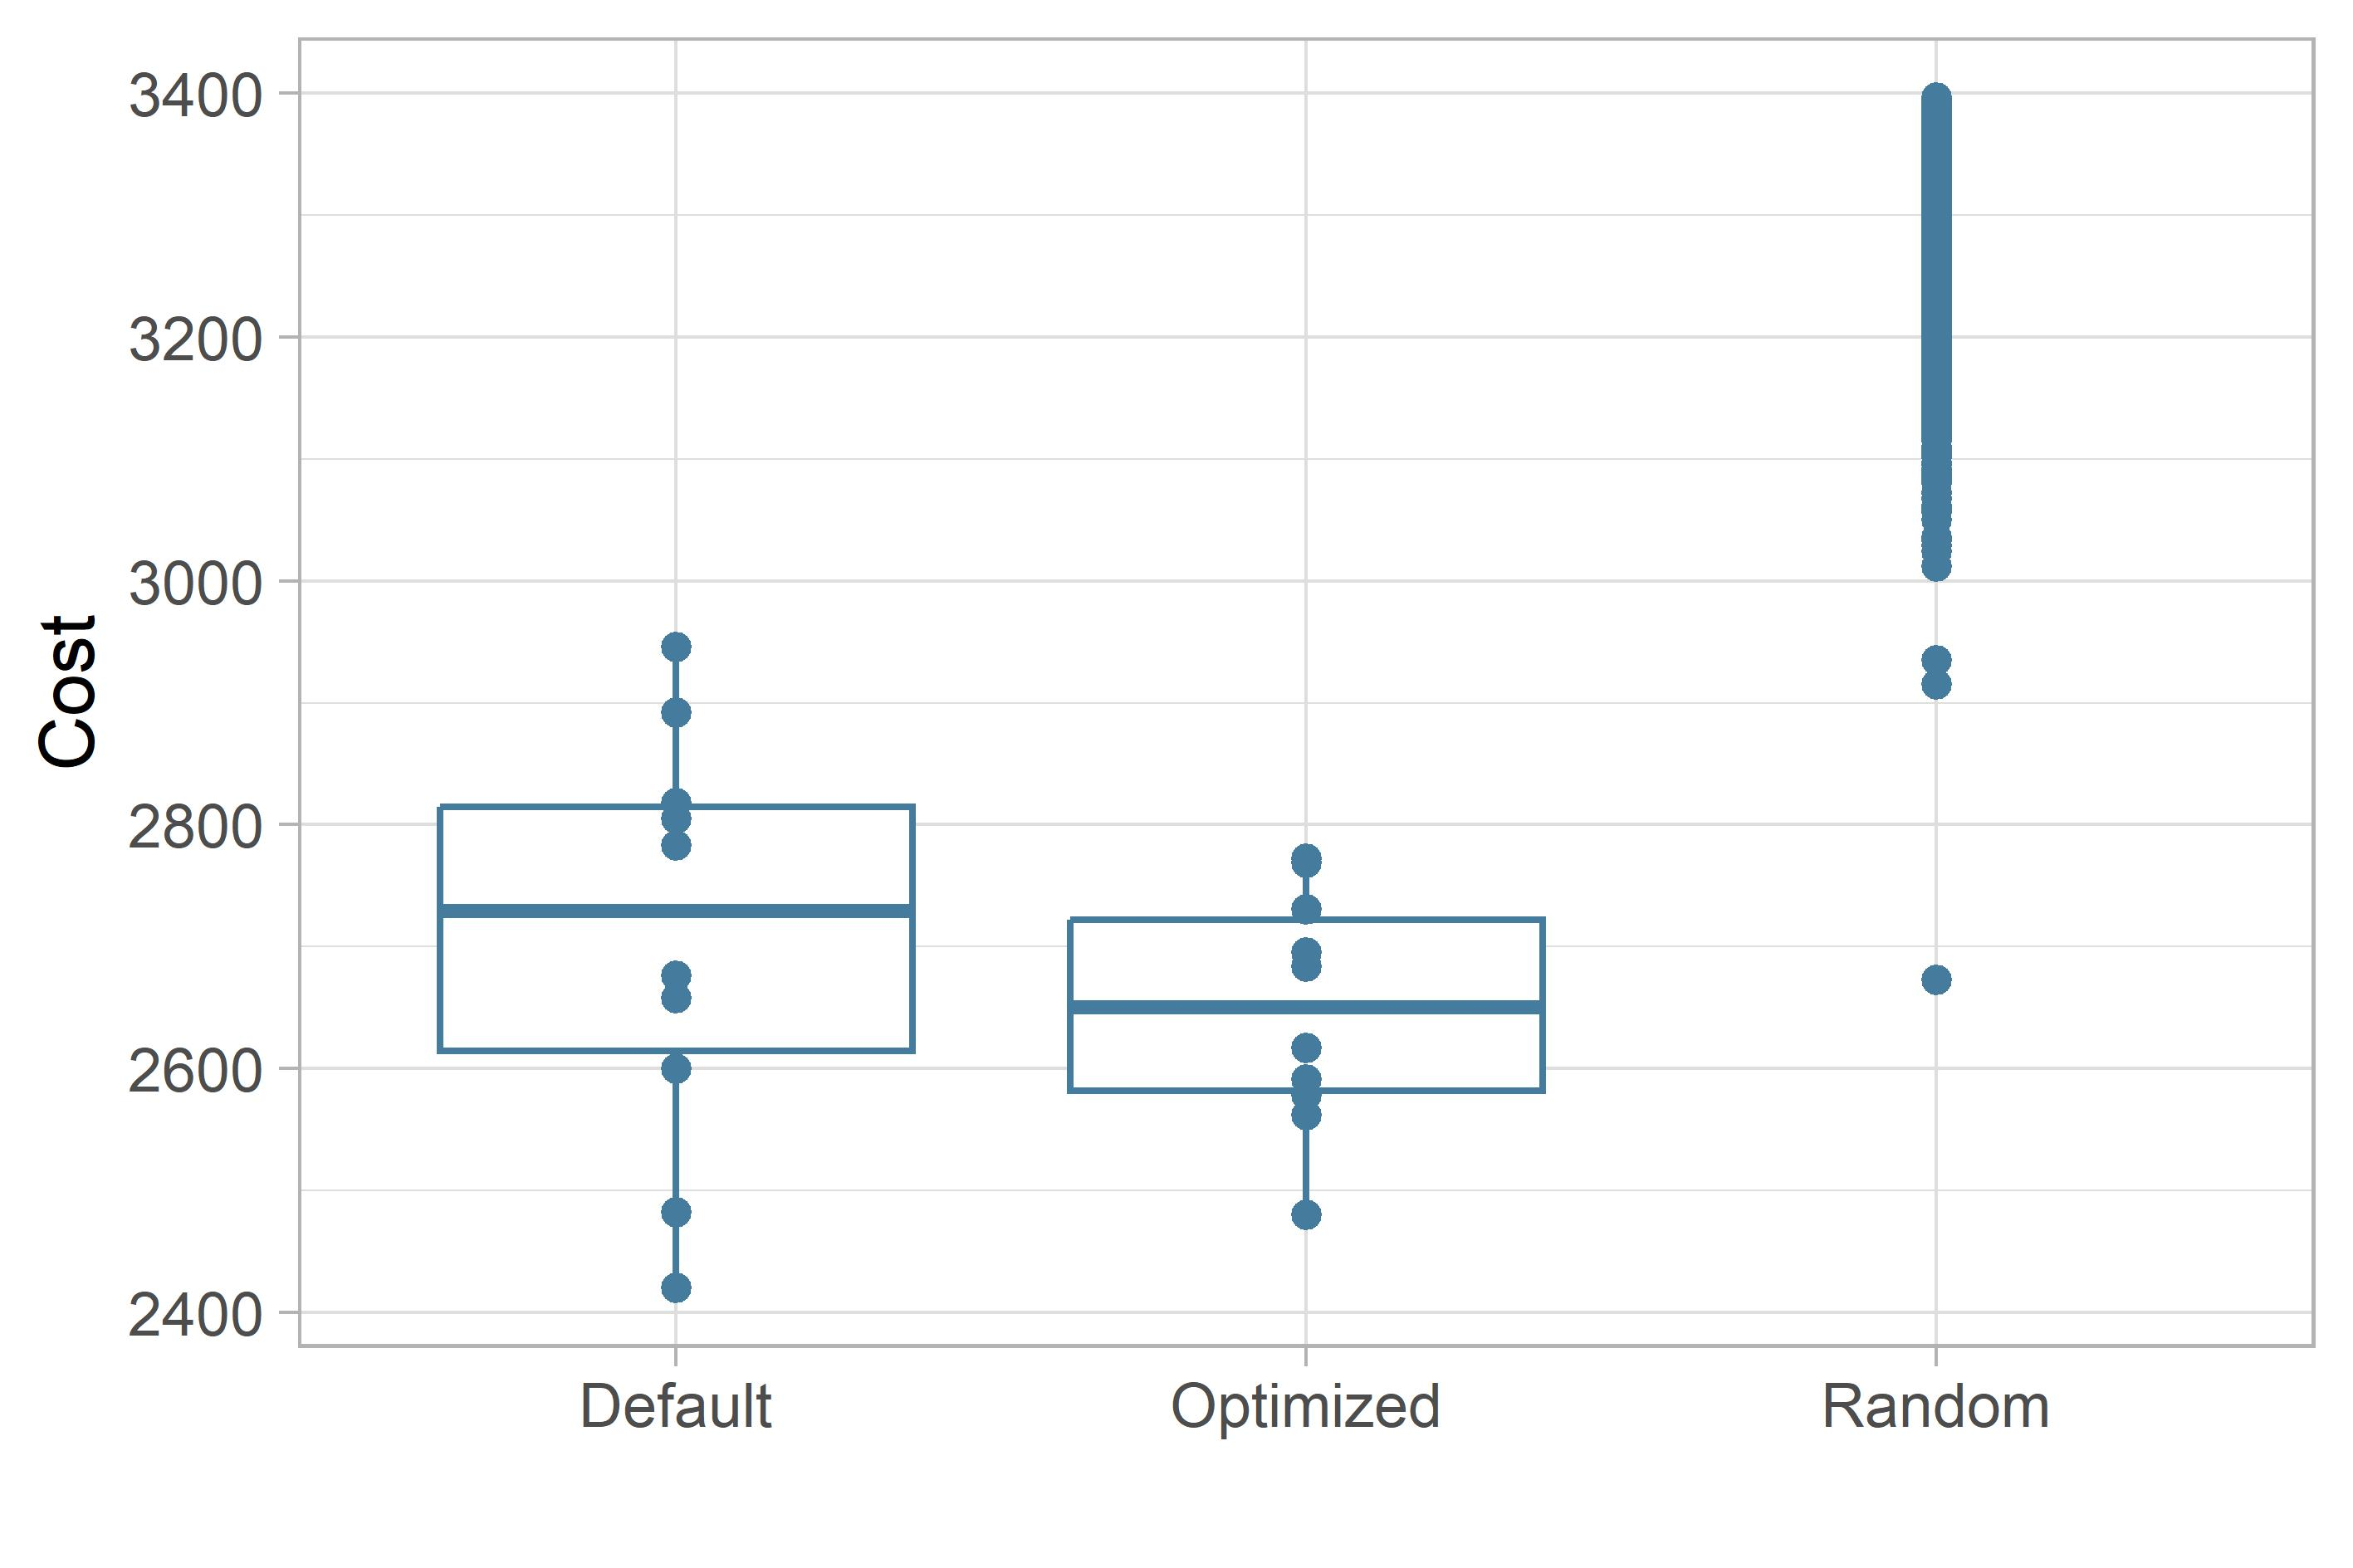
\includegraphics[width=1\linewidth]{simulations/evaluation/plots/sim_1_comparison}
	\caption{Start Scenario 1: Default GA vs Optimized GA vs Random Search}
\end{figure}

Analysing the graph, the Optimized GA clearly outperformed the Default GA as well as Random Search.

Welchs t-test shows that on average, greater fitness is achieved by using Optimized GA (M = 8.52, SE = ?) than from using Default GA (M = 7.09, SE = ?). This difference was significant \textit{t}(17.87) = 3.15, p < .01. It did represent a large effect r = 0.60.
Compared to Random (M = 4.943, SE = ?), the Optimized GA has even higher dominance, with a significant difference \textit{t}(16.9) = 7.12, p < .001 and a large effect r = 0.87.

The better performance of the Optimized GA was however unsurprising, as it was specifically trained on the used start scenario.

To further analyse both genetic algorithms, a look at their performance over the generations next to their diversity chart is of interest. Figure \ref{figure:sim_1_ga_comparison} plots the mean over 10 repetitions, the outline show the first and third quantiles.

\begin{figure}[ht] 
	\label{figure:sim_1_ga_comparison}
	\begin{minipage}[b]{0.5\linewidth}
		\centering
		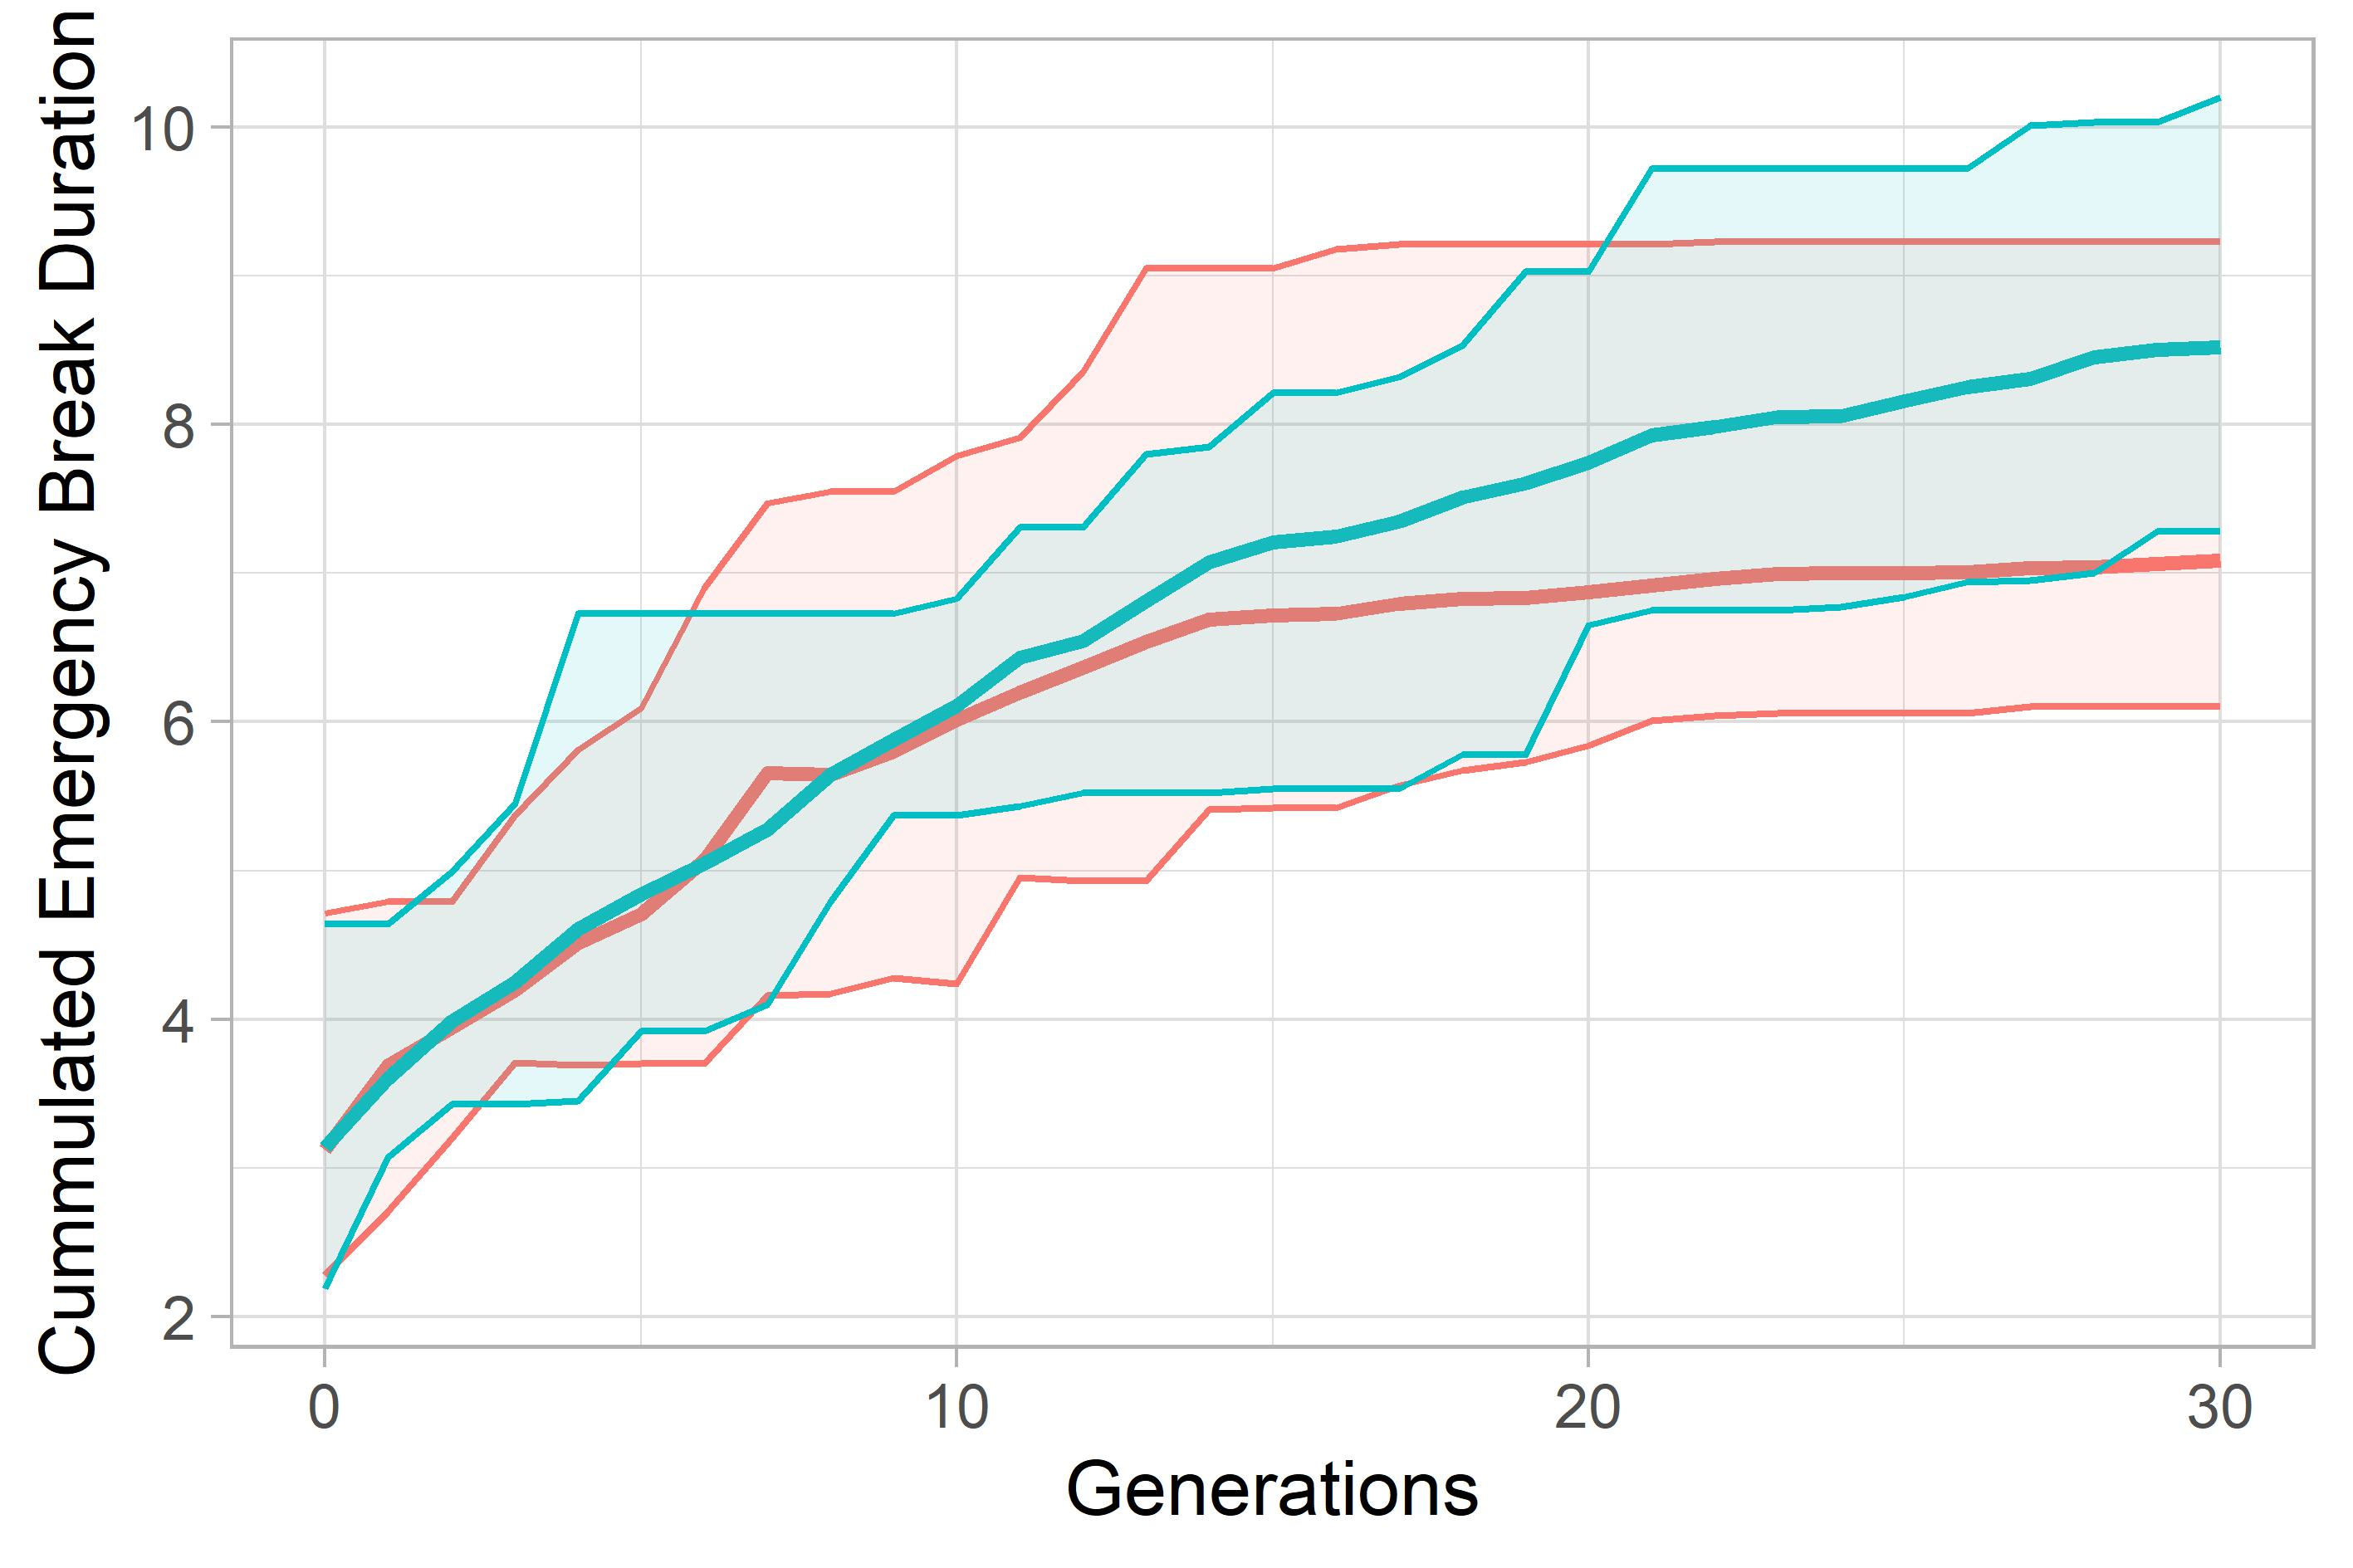
\includegraphics[width=1\linewidth]{simulations/evaluation/plots/sim_1_ga_generations} 
	\end{minipage}%%
	\begin{minipage}[b]{0.5\linewidth}
		\centering
		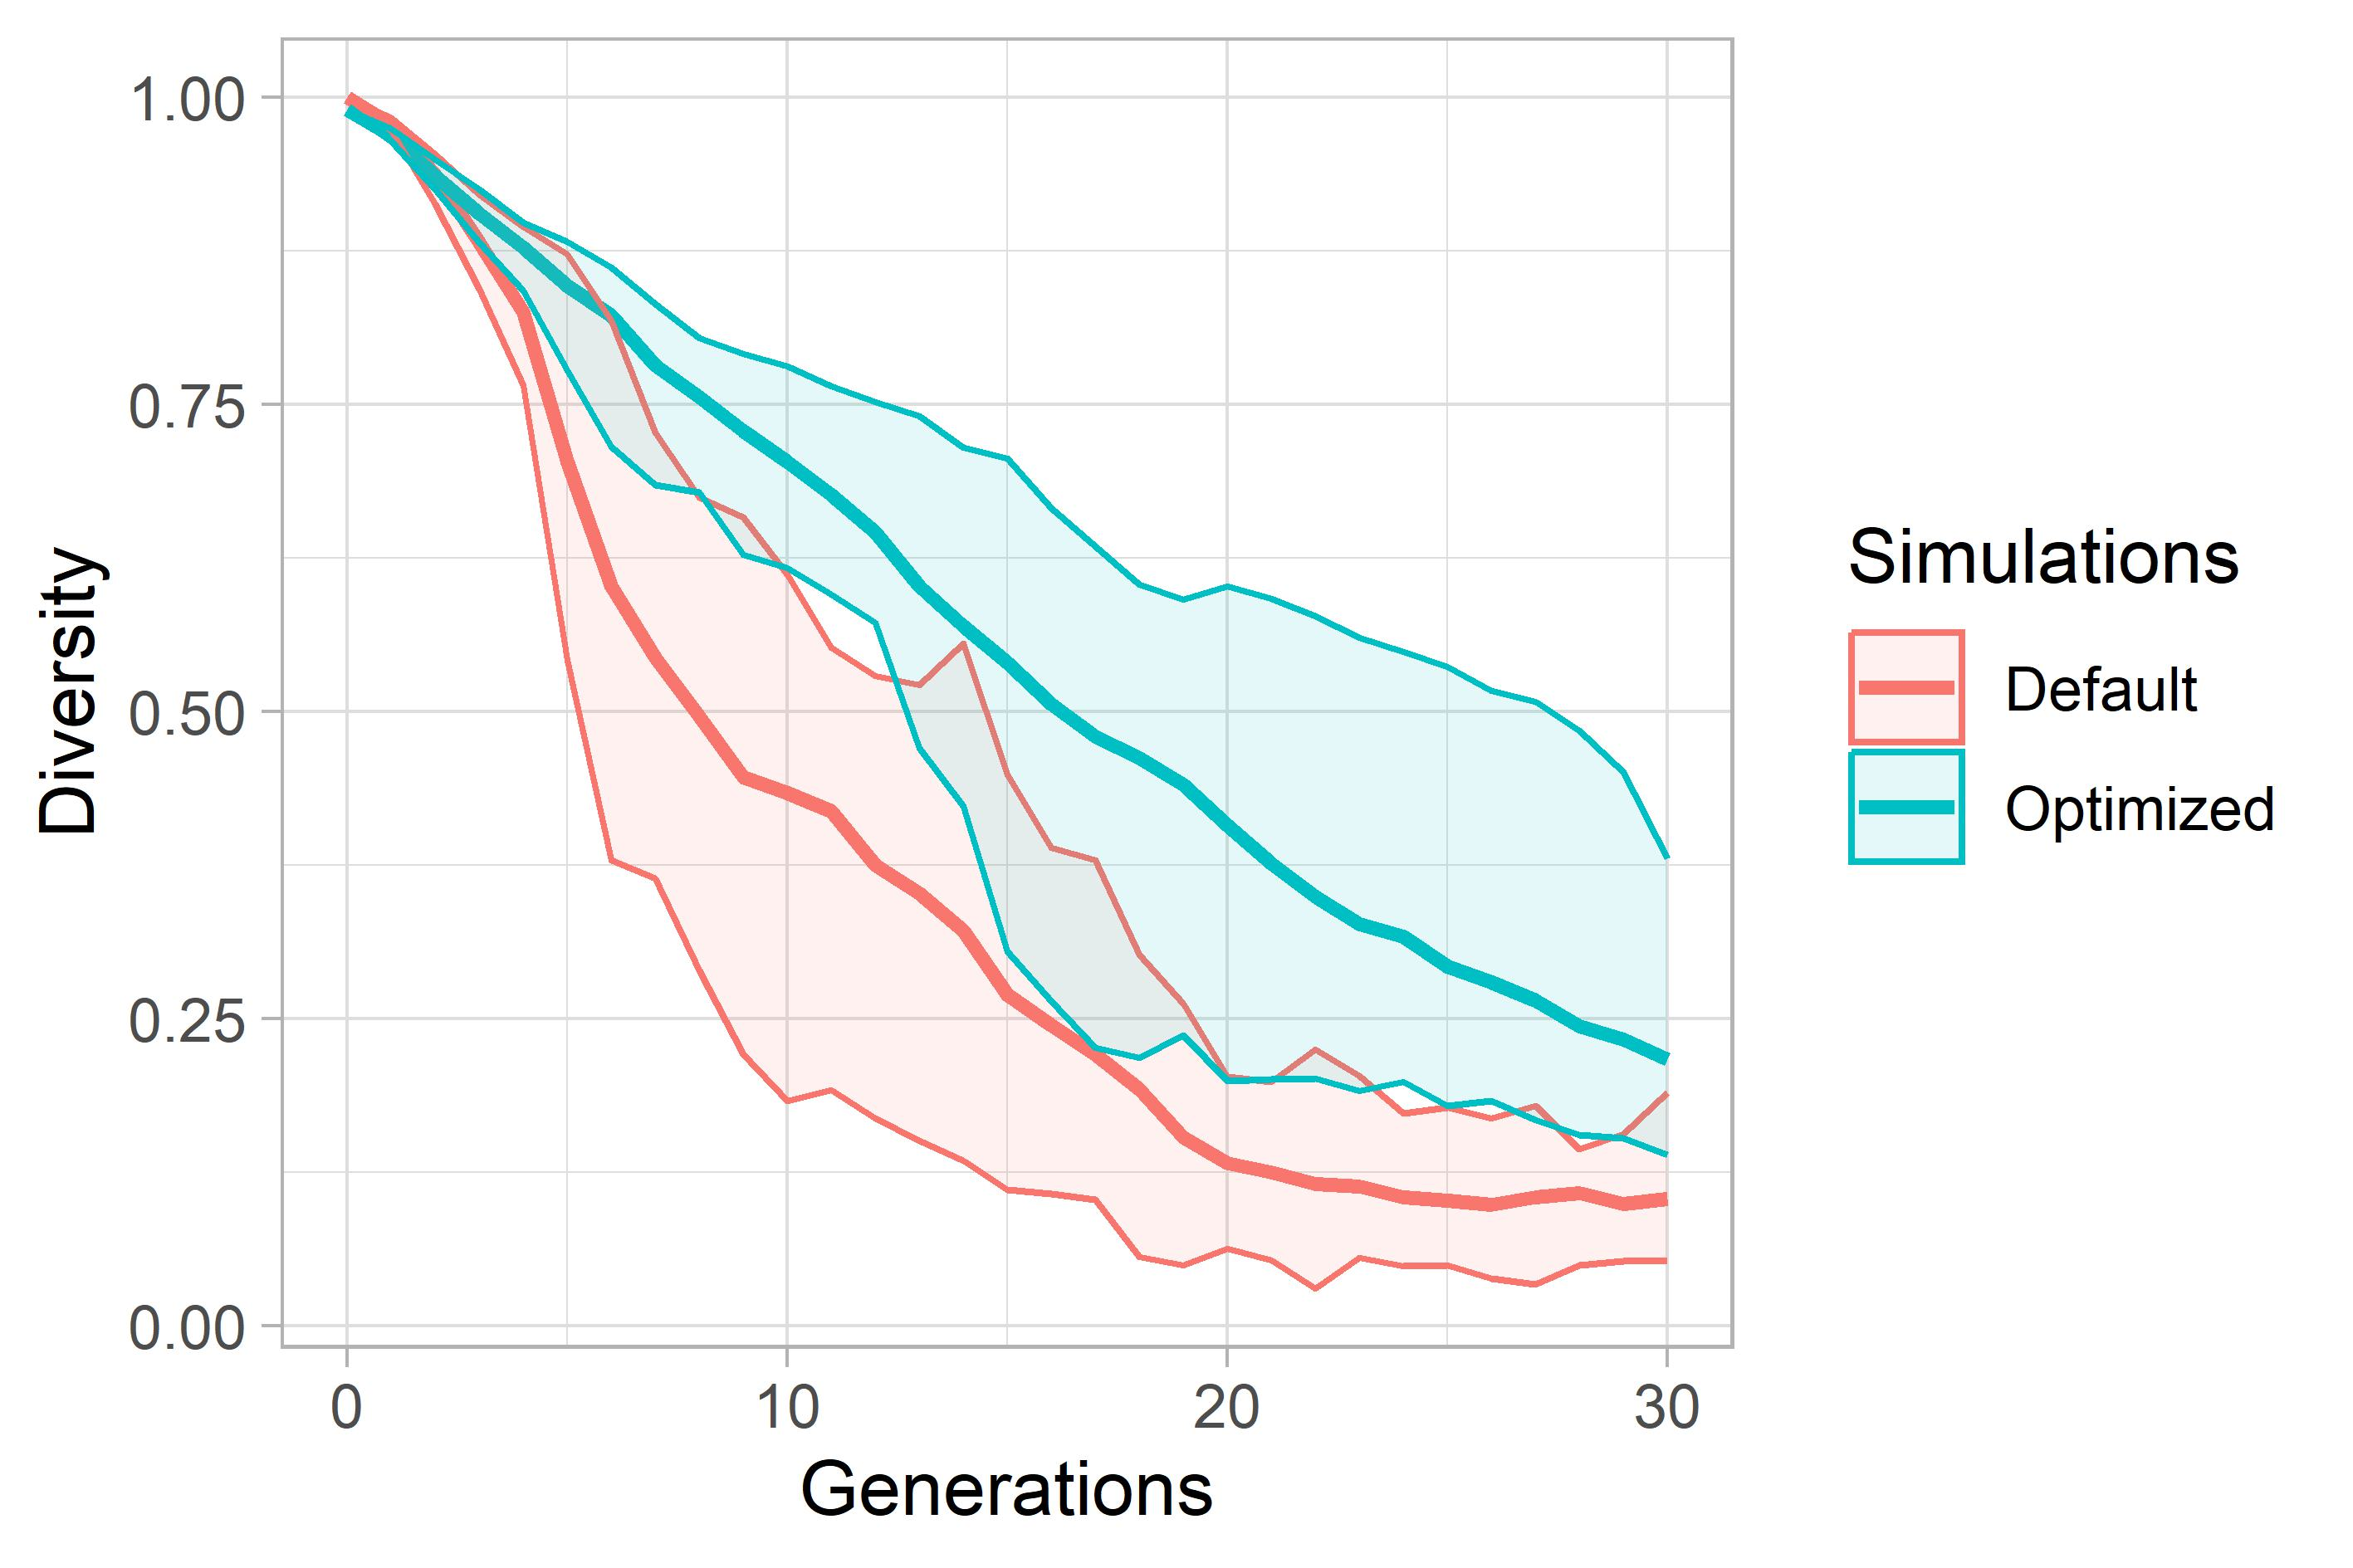
\includegraphics[width=1\linewidth]{simulations/evaluation/plots/sim_1_ga_diversity} 
	\end{minipage} 
	\caption{Start Scenario 1: Comparison of GAs}
\end{figure}

After generation 10, the rate of improved fitness of the Default GA drops compared to the Optimized GA. A combined early sharp decline in the diversity, suggests a connection. The Optimized GA shows to hold the diversity in the population longer, its rate of convergence is linear. Its high crossover and mutation rates seem to help with the improved diversity. The graph also shows, that a higher number of generations might not be useful for improved performance, as after 30 generations, the Optimized GA does not seem to hold enough diversity to continue with adequate performance gains. 

\section{Start Scenario 2}
9 Vehicles and 5 pedestrians. same number as start scenario 1.\todo{simulations have not yet finished}


\section{Start Scenario 3}
\label{chap:evaluation:scenario_3}
Start scenario 3 is described in more detail in Appendix \ref{figure:appednix:start_scenario_3}. 5 vehicles with 3 pedestrians are initialized, resulting in a simulation with only a small number of NPCs.

\begin{figure}[ht] 
	\label{figure:sim_3_comparison}
	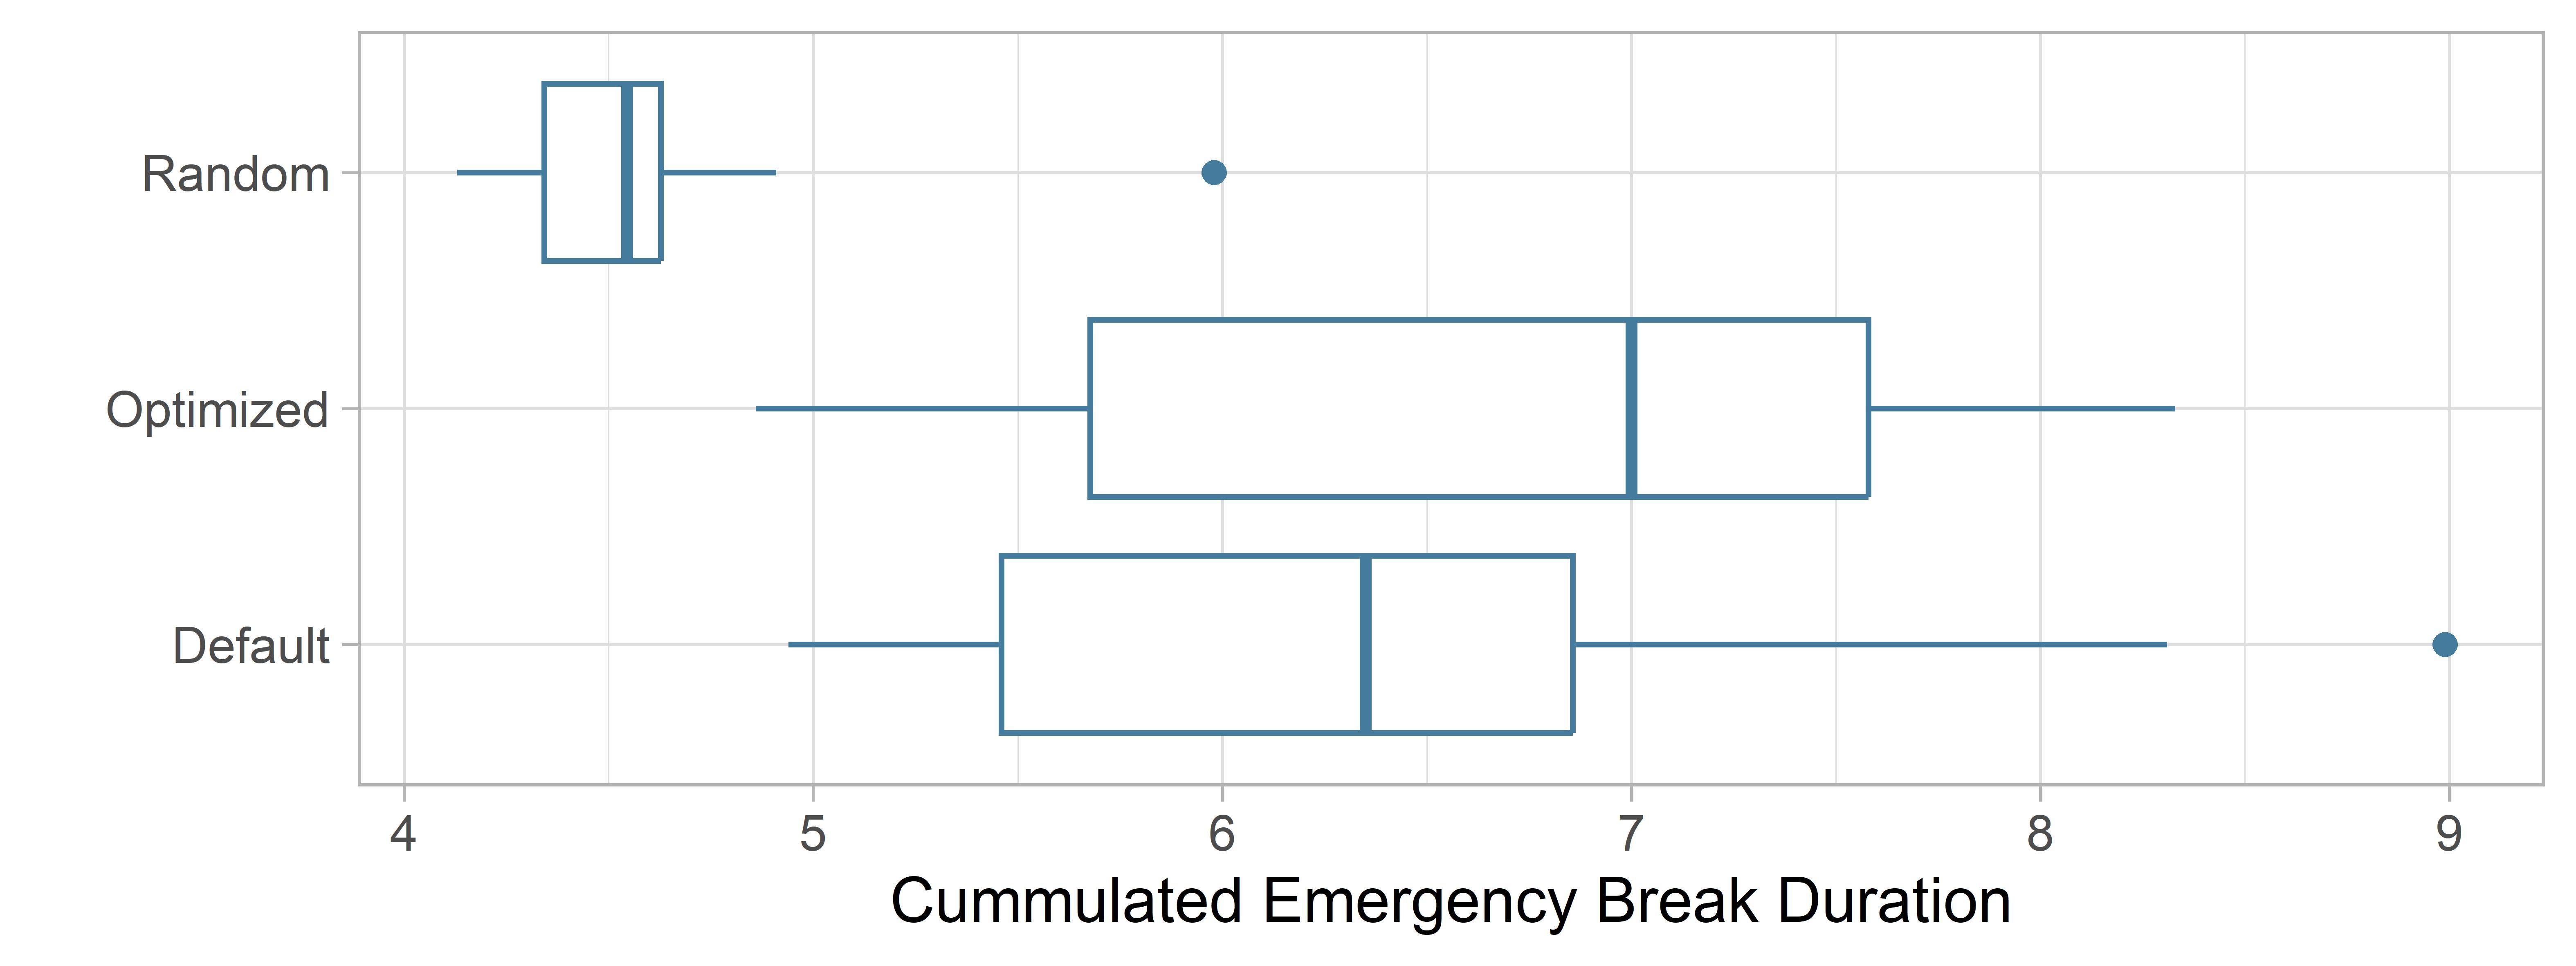
\includegraphics[width=1\linewidth]{simulations/evaluation/plots/sim_3_comparison}
	\caption{Start Scenario 3: Default GA vs Optimized GA vs Random Search}
\end{figure}

Looking at the graph, the Optimized GA again outperforms the Random Search, however there seams to be only marginal improvements compared to Default GA. 

A t-test confirms these findings. While on average, greater fitness is achieved by using Optimized GA (M = 6.66, SE = ?) than from using Default GA (M = 6.49, SE = ?). This difference was however not significant \textit{t}(17.83) = 0.29, p > .05 and an effect size of r = 0.07.
Verifying the better performance of the Optimized GA compared to Random Search (M = 4.619, SE = ?) shows a significat difference \textit{t}(12.4) = 4.9, p < .001 and a large effect size of r = 0.81.

To further analyse both genetic algorithms, their performance over the generations next to their diversity chart is again shown in figure \ref{figure:sim_3_ga_comparison}. The mean over 10 repetitions is plotted, the outline show the first and third quantiles.

\begin{figure}[ht] 
	\label{figure:sim_3_ga_comparison}
	\begin{minipage}[b]{0.5\linewidth}
		\centering
		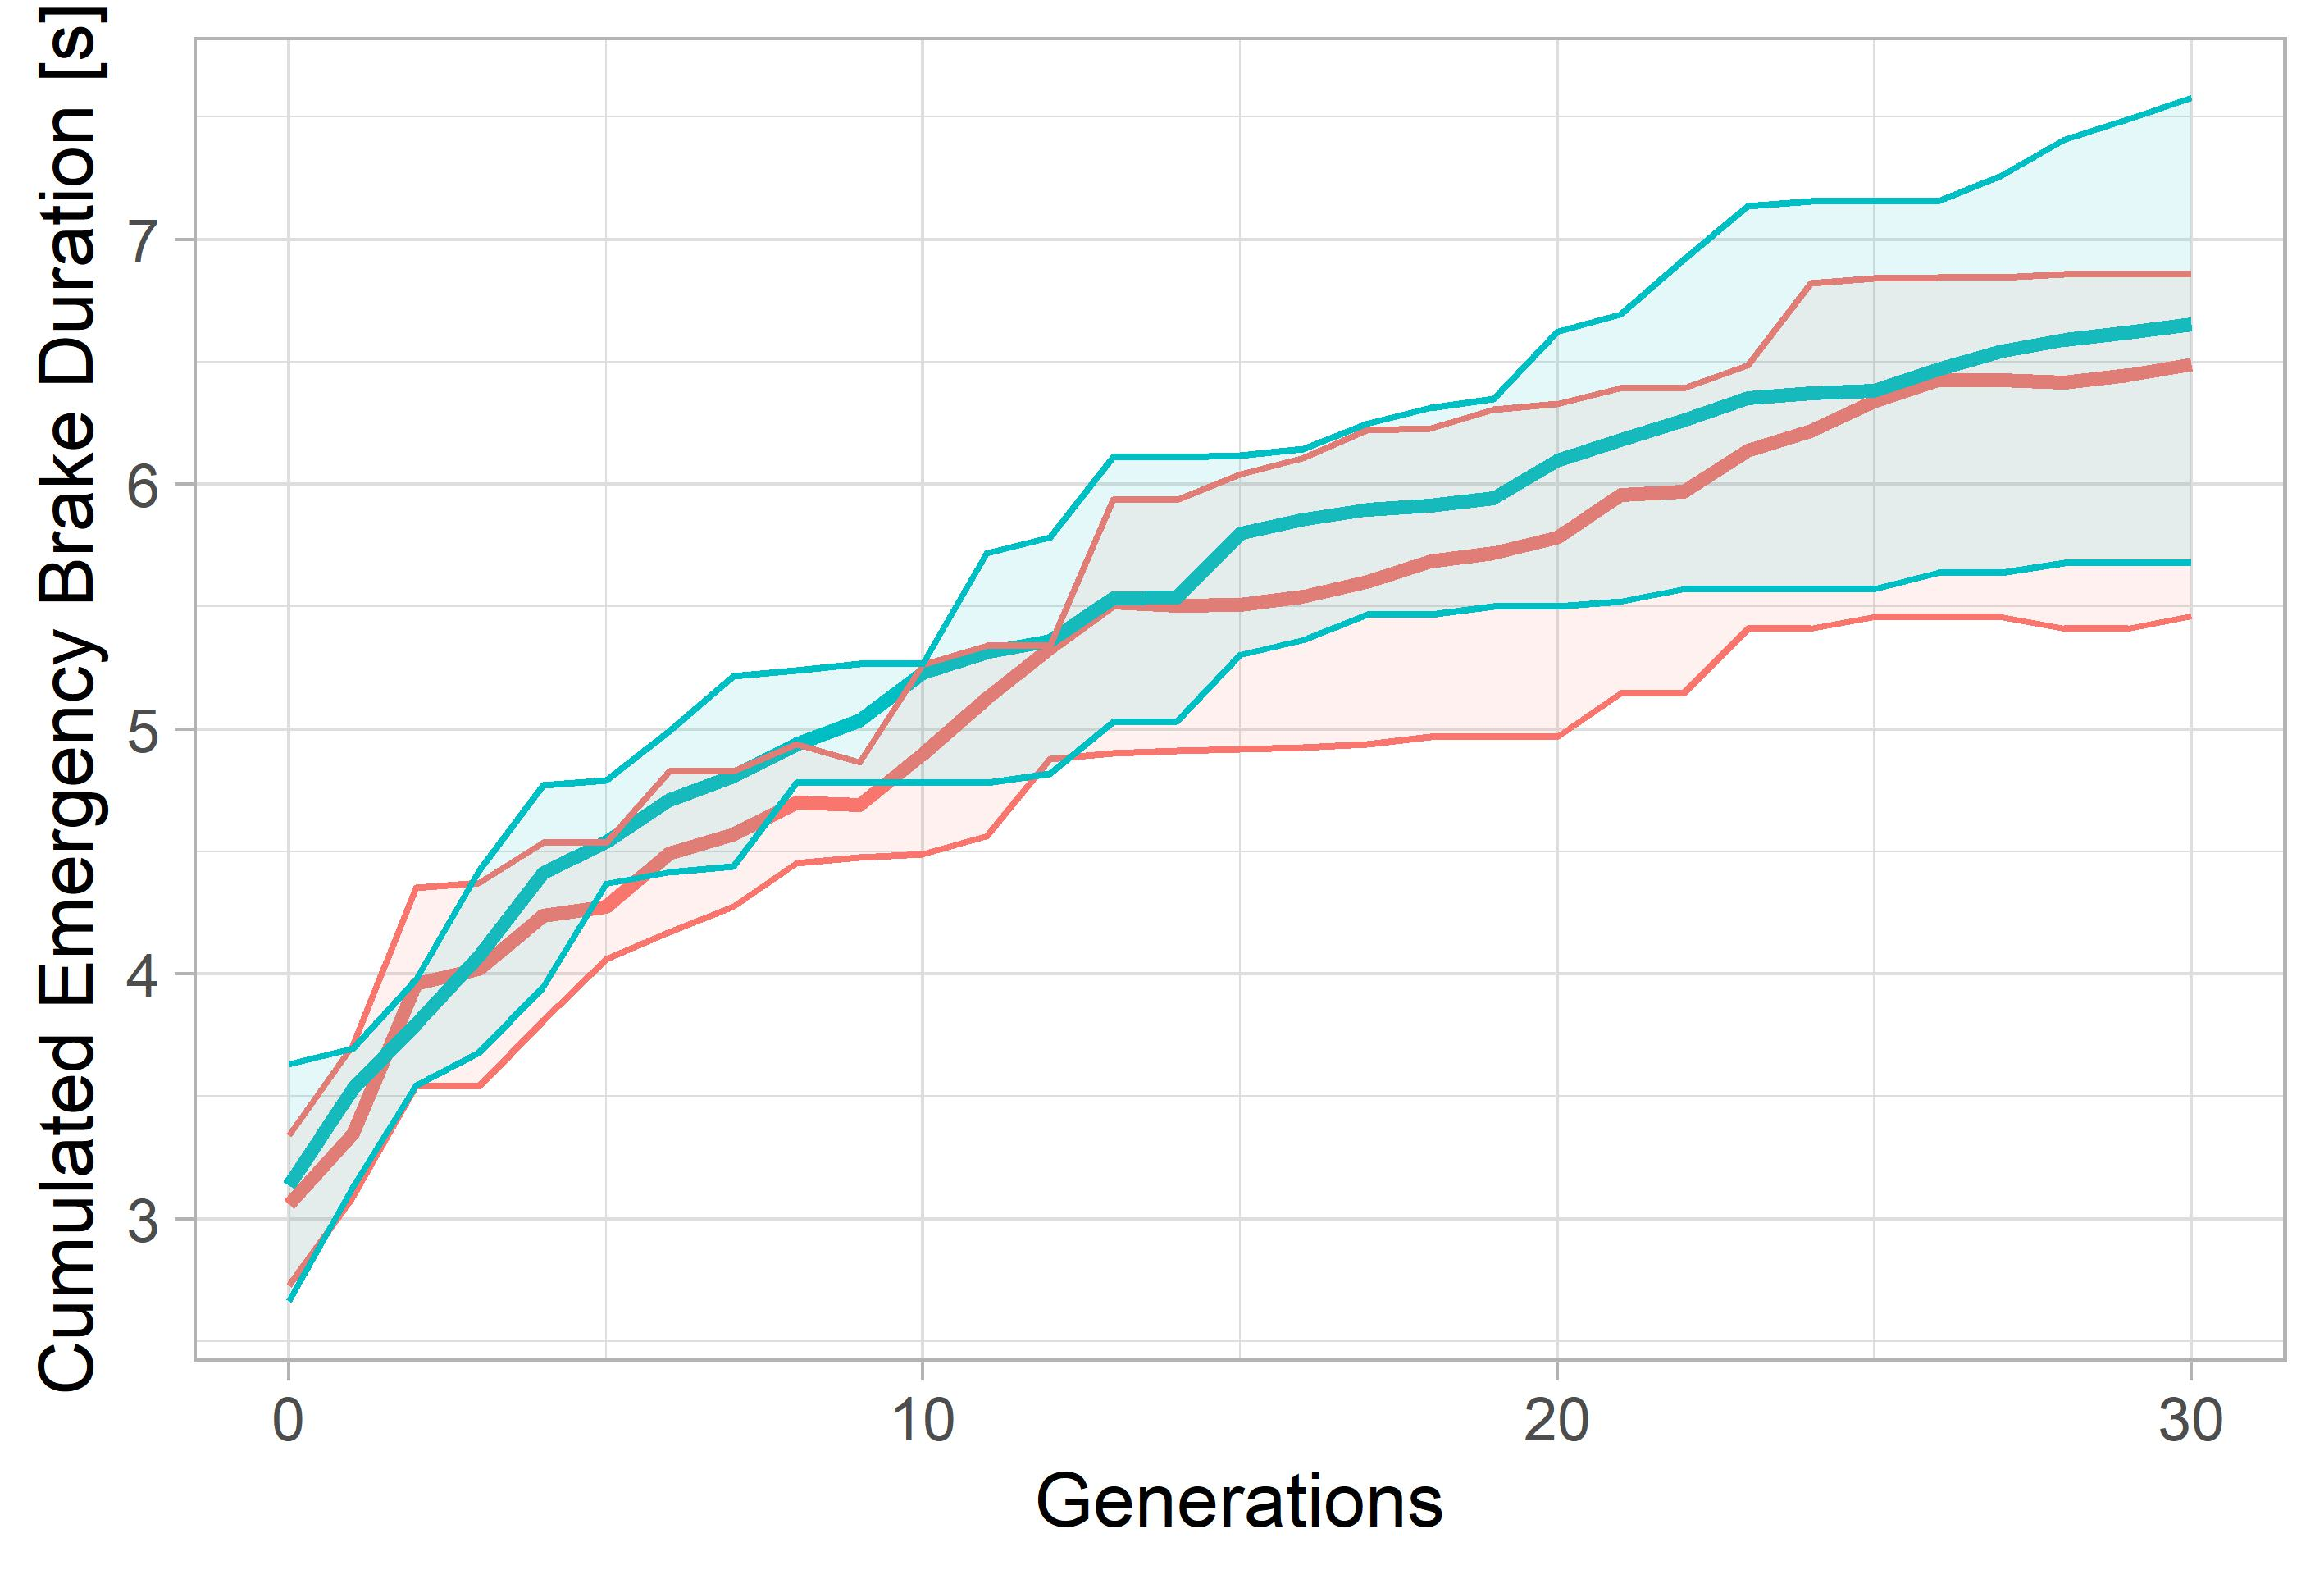
\includegraphics[width=1\linewidth]{simulations/evaluation/plots/sim_3_ga_generations} 
	\end{minipage}%%
	\begin{minipage}[b]{0.5\linewidth}
		\centering
		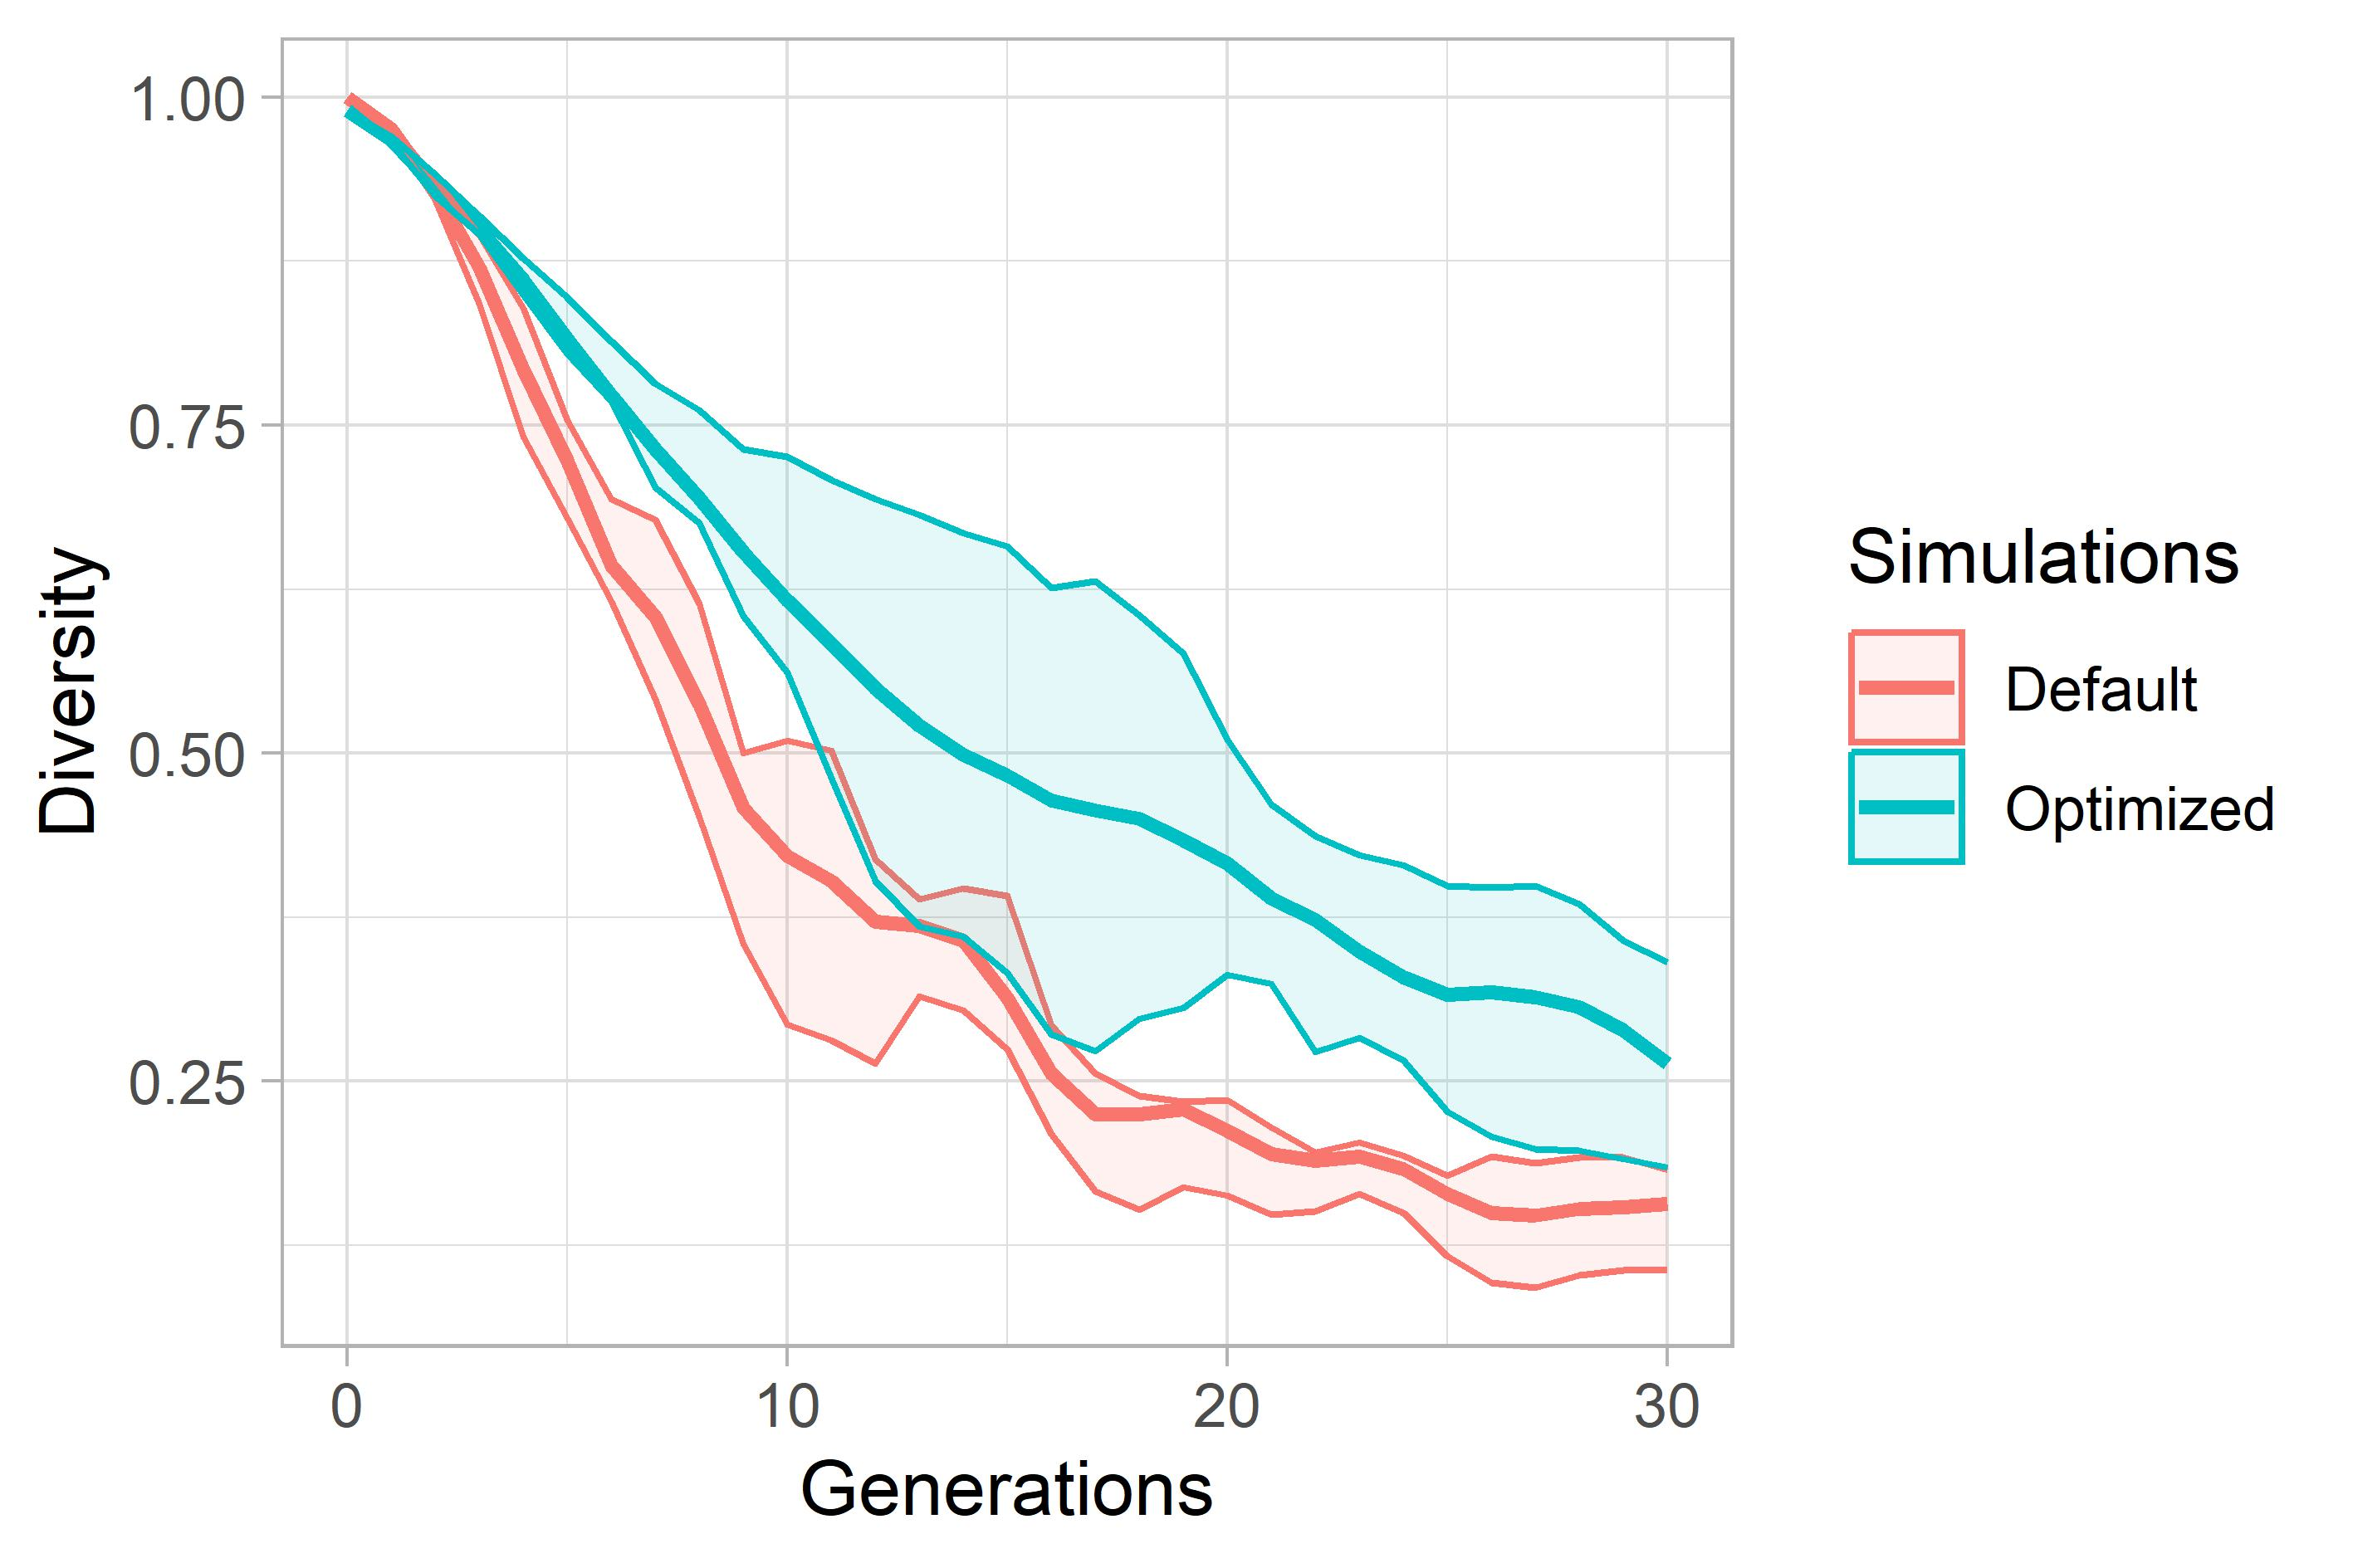
\includegraphics[width=1\linewidth]{simulations/evaluation/plots/sim_3_ga_diversity} 
	\end{minipage} 
	\caption{Start Scenario 3: Comparison of GAs}
\end{figure}


The rate of improved fitness of the Default GA now drops very similar to the Optimized GA. The early decline in the diversity is also not as pronounced as in the previous comparisons. While the optimized GA shows to still hold the diversity in the population longer, this only has a minimal impact on its average fitness. The similarity in performance might be explained by the smaller search space due to the smaller number of NPCs. Here, high mutation and crossover rates might not have the previous pronounced advantage.

\section{Start Scenario 4}
Start scenario 4 can be seen in Appendix at \ref{figure:appednix:start_scenario_4}. 18 vehicles with 10 pedestrians are initialized, resulting in the simulation with the most NPCs.

\begin{figure}[ht] 
	\label{figure:sim_4_comparison}
	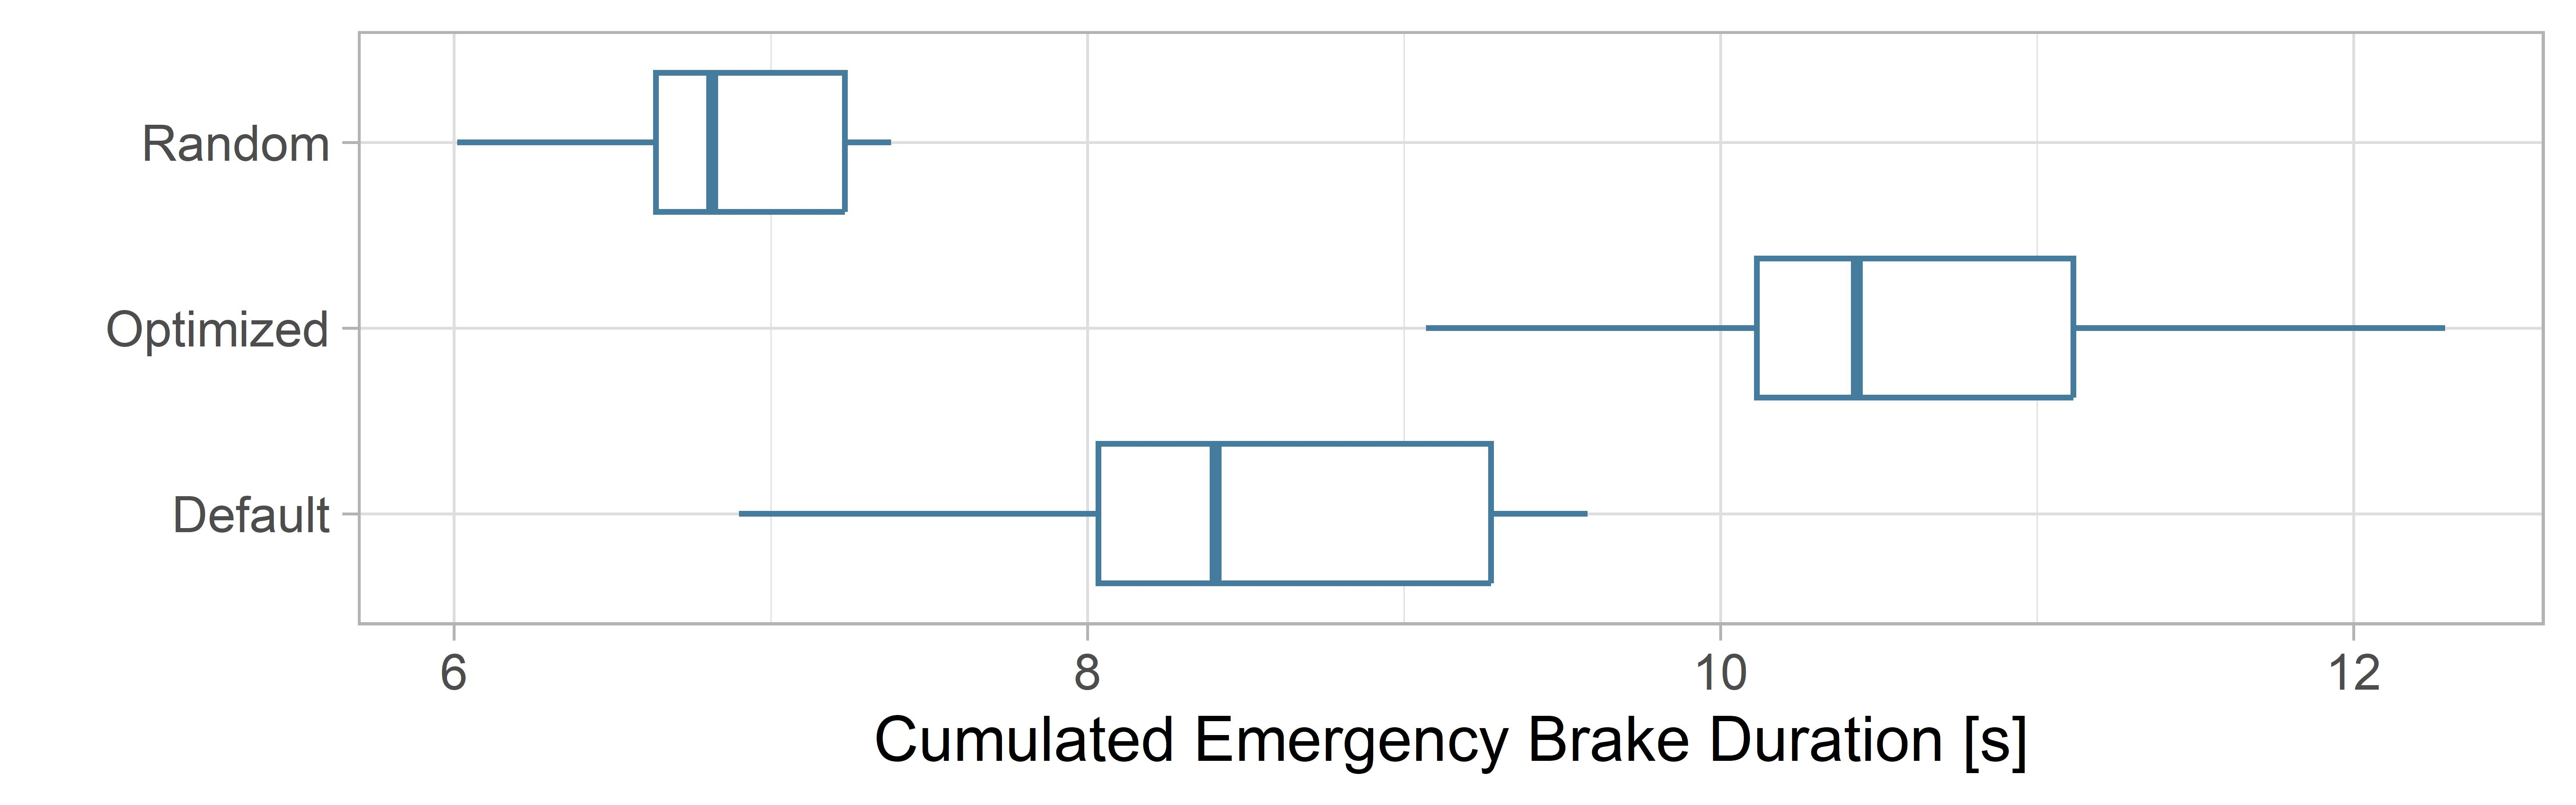
\includegraphics[width=1\linewidth]{simulations/evaluation/plots/sim_4_comparison}
	\caption{Start Scenario 4: Default GA vs Optimized GA vs Random Search}
\end{figure}

Figure \ref{figure:sim_4_comparison} shows the Optimized GA clearly outperforming the Default GA as well as Random Search.
The Optimized GA (M = 10.60, SE = ?) has significantly greater fitness then the Default GA (M = 8.46, SE = ?) with \textit{t}(17.98) = 5.30, p < .001 and a large effect r = 0.78.
Compared to Random Search (M = 6.86, SE = ?), the greater fitness of the Optimized GAs is significant with \textit{t}(11.71) = 12.7, p < .001 and a large effect r = 0.96.

Both genetic algorithms performance over the generations next to their diversity chart is compared in figure \ref{figure:sim_4_ga_comparison}.

\begin{figure}[ht] 
	\label{figure:sim_4_ga_comparison}
	\begin{minipage}[b]{0.5\linewidth}
		\centering
		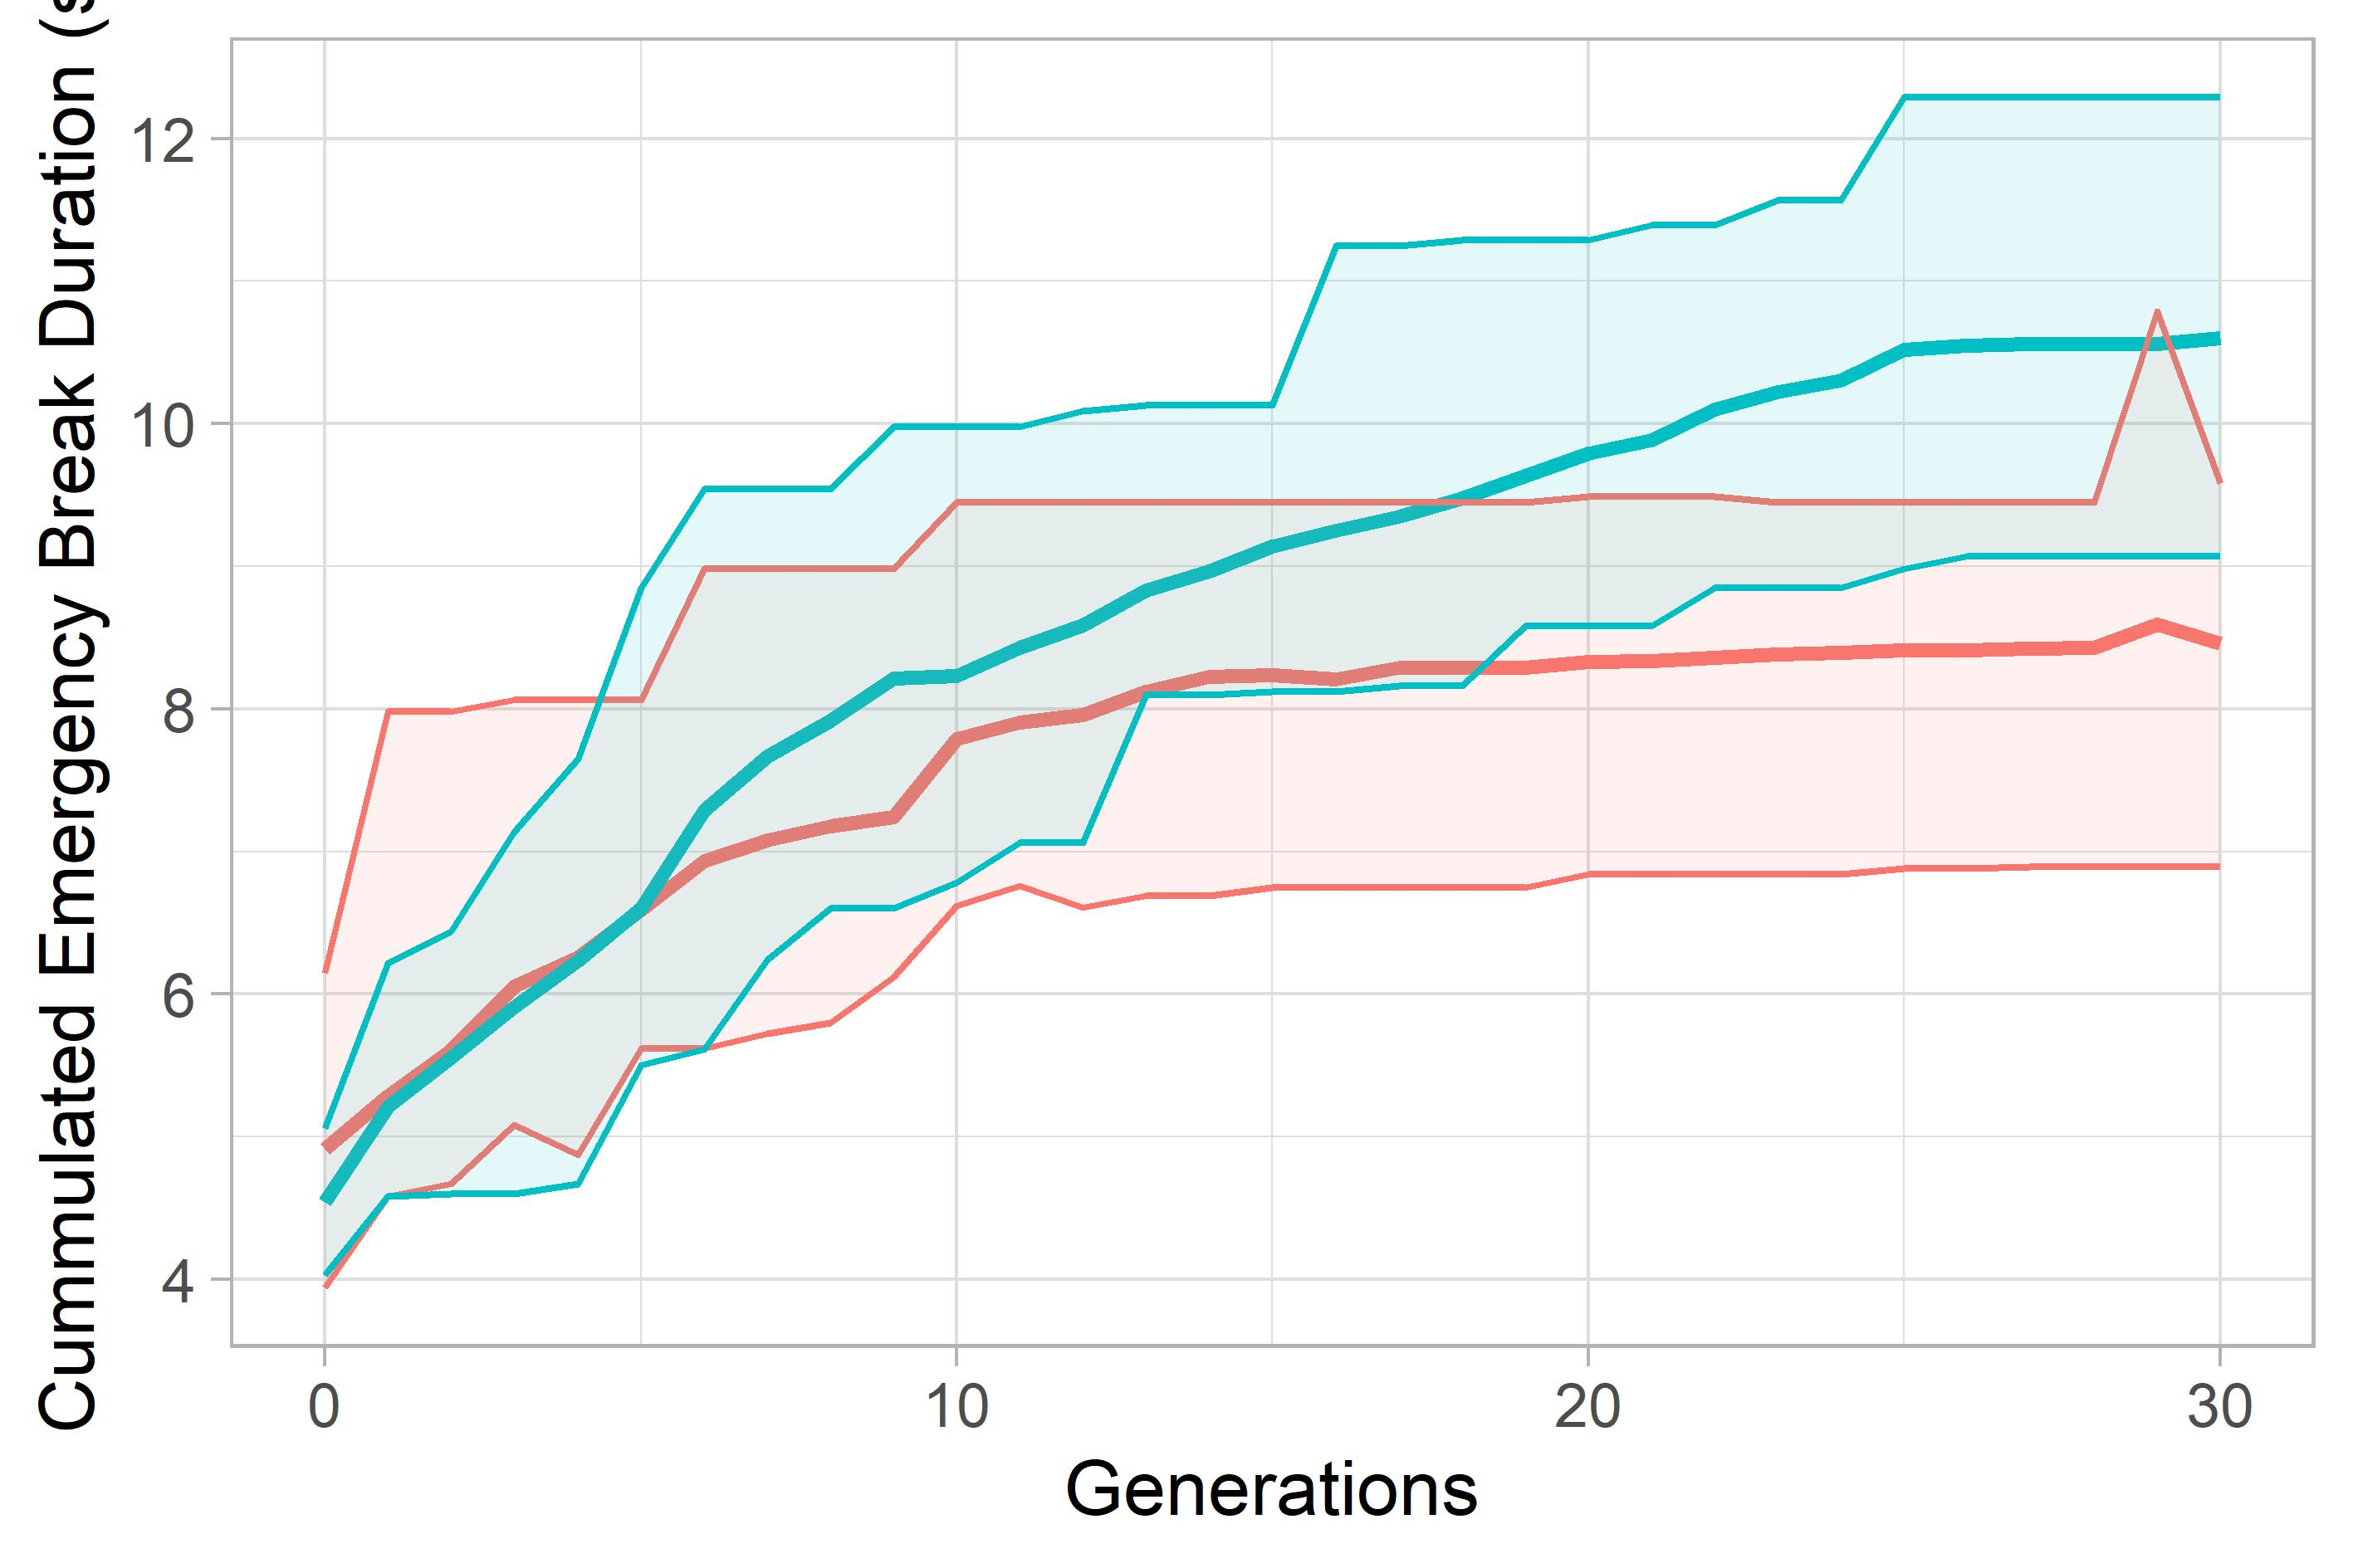
\includegraphics[width=1\linewidth]{simulations/evaluation/plots/sim_4_ga_generations} 
	\end{minipage}%%
	\begin{minipage}[b]{0.5\linewidth}
		\centering
		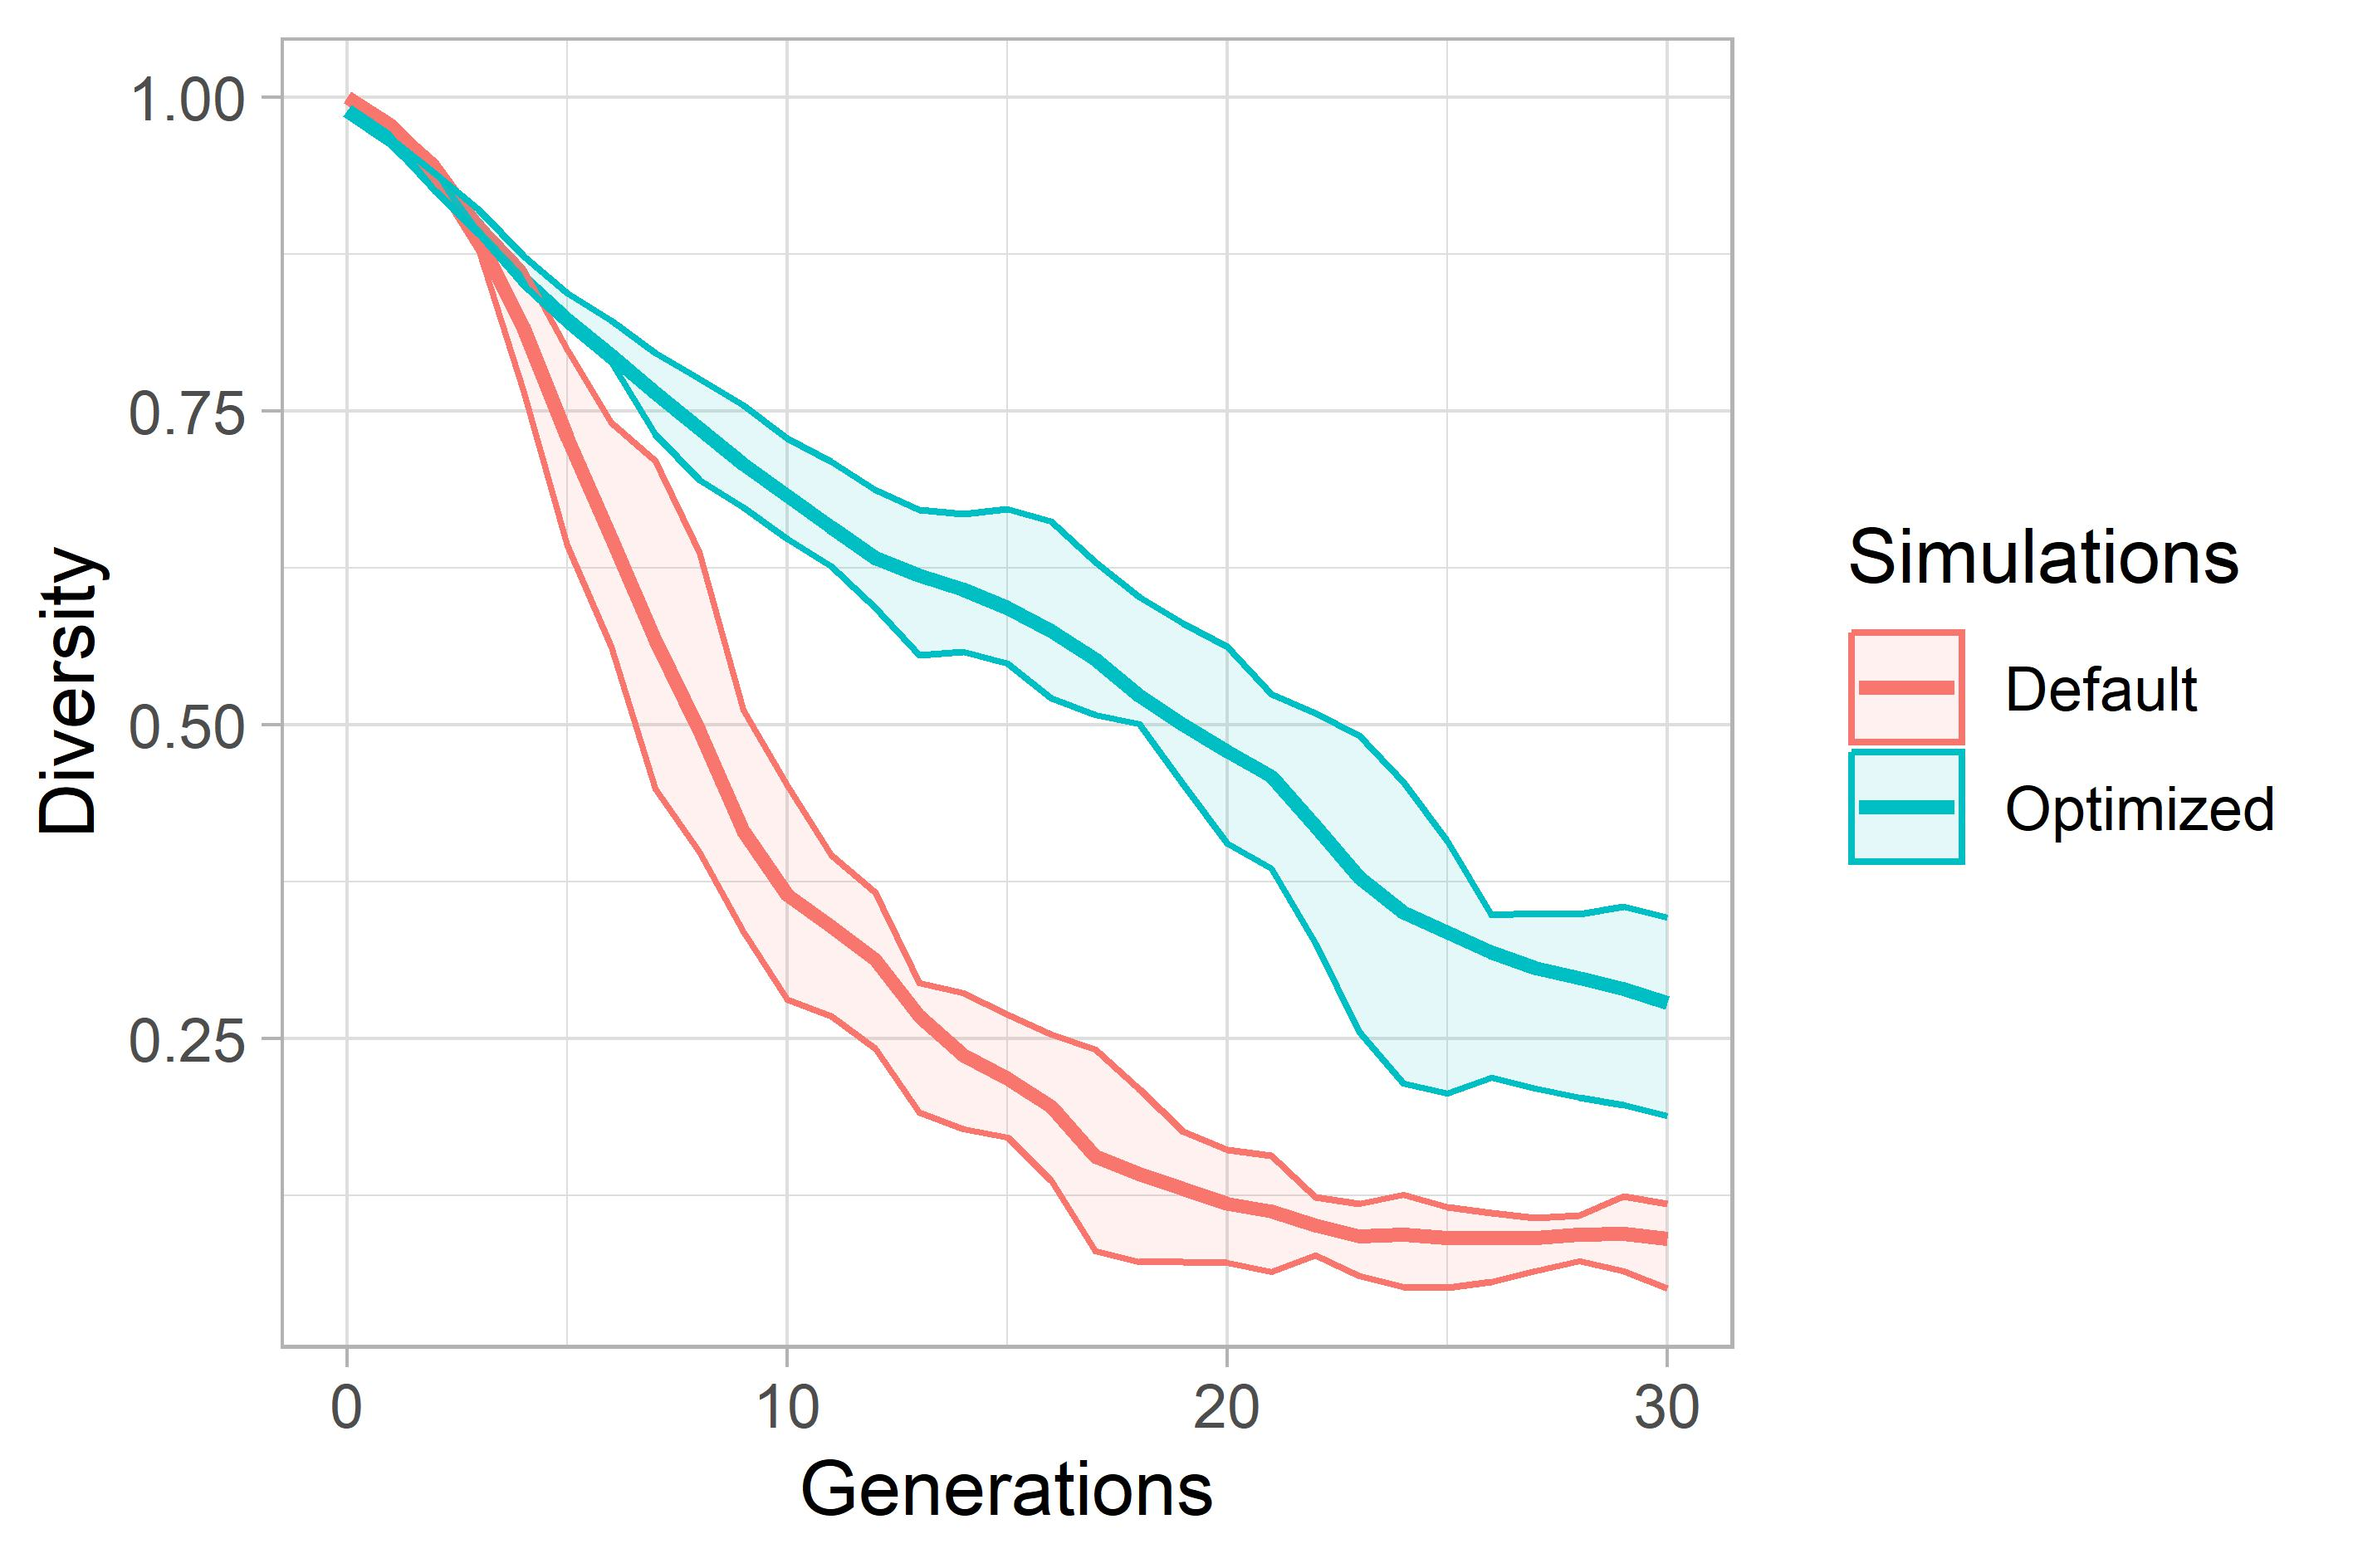
\includegraphics[width=1\linewidth]{simulations/evaluation/plots/sim_4_ga_diversity} 
	\end{minipage} 
	\caption{Start Scenario 4: Comparison of GAs}
\end{figure}


Already at generation 5, the average rate of improved fitness of the Default GA drops compared to the Optimized GA. This is accompanied by an early sharp decline in the diversity. The optimized GA again shows be able to hold the diversity much longer at a high level, its rate of diversity drop is linear.
The results underline the statement made in section \ref{chap:evaluation:scenario_3}, which claims, that the Optimized GA excels at scenarios with lots of NPCs, where a vast search space is given.



